\documentclass[Rapport/Rapport_main.tex]{subfiles}
\begin{document}
\subsection{Softwarearkitektur}

\subsubsection{playerSideApp}
I det følgende afsnit beskrives softwarearkitekturen for \textbf{playerSideApp}. Denne applikation skal køre på en PSoC og skal derfor udvikles i C, men der laves stadig en  applikationsmodel opbygget som klasser, som implementeres som separate moduler (separate header- og implementeringsfiler). Der er til applikationsmodellen udviklet et klassediagram, en tilstandsmaskine og to sekvensdiagrammer. Alle disse samt detaljeret beskrivelse af diagrammer, klasser, funktioner og attributter kan ses i dokumentet \textbf{Arkitektur} afsnit \fullref{arch:sec:playersideapp_application_model}.\\\\
Den vigtige del af denne applikationsmodel er klassediagrammet og tilstandsmaskinen. Klassediagrammet kan ses på figur \ref{fig:CD_PlayerSide}.

\begin{figure}[H]
    \centering
    \centering
    \makebox[\textwidth][c]{%
        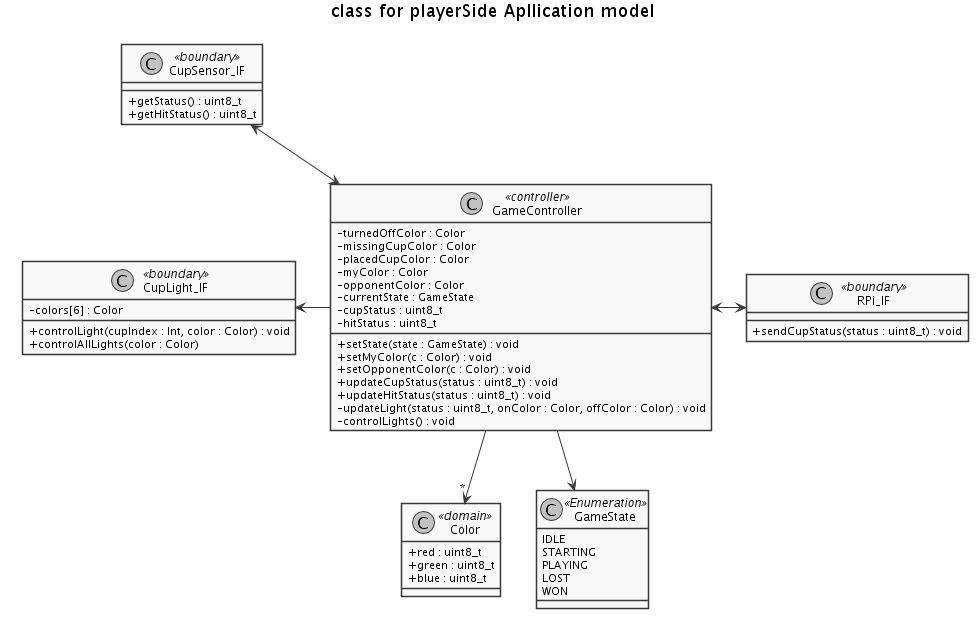
\includegraphics[width=1.2\textwidth]{Arkitektur/Softwarearkitektur/Applikationsmodel/PlayerSide/graphics/classDiagram.png}
    }
    \caption{Klassediagram for \textbf{playerSideApp}}
    \label{fig:CD_PlayerSide}
\end{figure}
Boundary klasserne er bestemt ud fra de relevante hardwareblokke som PSoC Player side er forbundet til. Disse klasser slutter på '\_IF', for interface. CupLight\_IF og CupSensor\_IF har tilsammen ansvar for at styre alle Cup Holders. Derudover er der klassen RPi\_IF, som har til ansvar for at styre kommunikation til og fra RPi blokken. Color er en domæneklasse, som indeholder information om farver og fremkommer af en analyse af kravspecifikationen. Fra kravspecifikationen er de tre Use Cases UC1, UC2 og UC3 relevante for \textbf{playerSideApp}. Klassen GameController kombinerer disse tre Use Cases, og har til ansvar at styre Cup Lights og sende data til RPi. Cup lights skal styres på baggrund af hvilke kopper, der placeres og hvilke, der rammes, og afhænger af hvilken tilstand og hvilke farver (myColor og opponentColor), der modtages fra RPi. Derudover skal den også sende information, om hvilke kopper der er placeret til RPi.\\

Der er også en blok GameState, som beskriver de forskellige tilstande, applikationen kan have. De fremgår i tilstandsmaskinen, som ses på figur \ref{fig:playerSide_SM}. Det ses på diagrammet, at tilstandsmaskinen skifter tilstand, når der kaldes metoden setState. Denne metode kaldes af RPi\_IF klassen, når der modtages en ny tilstand. Controller funktionen styrer lyset på baggrund af tilstanden og attributterne cupStatus og hitStatus. Der er til UC1 og UC2 udviklet sekvensdiagrammer, som kan ses i afsnit \autoref{arch:sec:playersideapp_application_model} i \textbf{Arkitektur} bilaget.      

\begin{figure}[H]
    \centering
    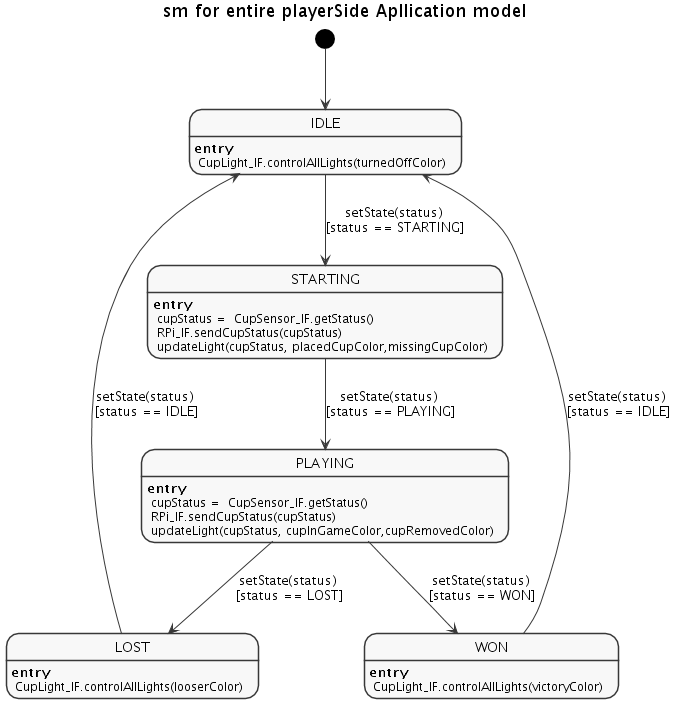
\includegraphics[width=0.9\textwidth]{Arkitektur/Softwarearkitektur/Applikationsmodel/PlayerSide/graphics/state.png}
    \caption{Tilstandmaskine for \textbf{playerSideApp}}
    \label{fig:playerSide_SM}
\end{figure}


\subsubsection{RPiApp}
I det følgende afsnit beskrives softwarearkitekturen for RPiApp. Den fulde dokumentation for RPiApp kan ses i bilaget \textbf{Arkitektur} i afsnit \fullref{arch:sec:rpiapp_application_model}. \\
Softwareapplikationen består af forskellige sprog, men generelt er objektorienteret C++ benyttet. I forlængelse af dette er der lavet en applikationsmodel til at beskrive strukturen og forløbet for applikationens objekt-orienteret softwaresystem. I de næste afsnit ses klasse- og sekvensdiagrammer for use case 1. \\\\
\textbf{Klassediagram}\\
Nedenfor ses klassediagrammet for UC1 til UC4. 
\begin{figure}[H]
    \centering
    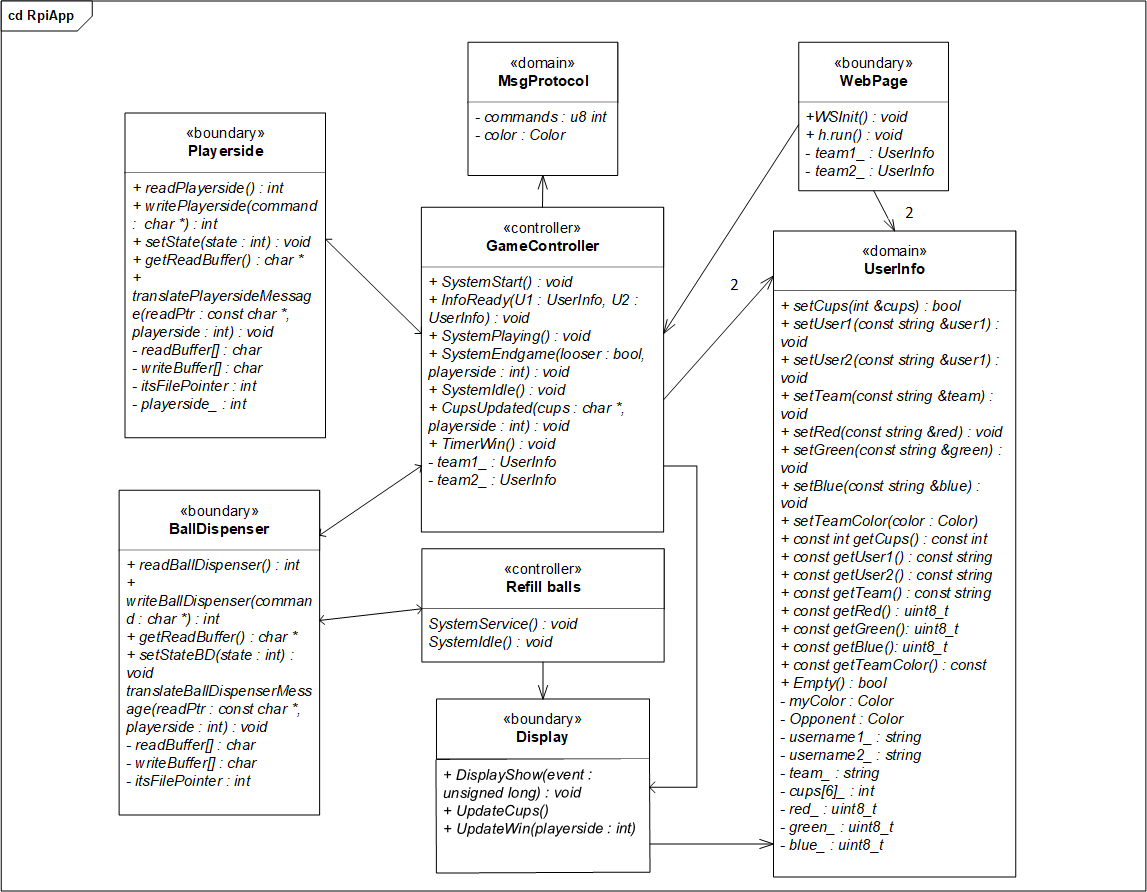
\includegraphics[width=\textwidth]{Arkitektur/Softwarearkitektur/Applikationsmodel/RPi/graphics_RPi/Class.png}
    \caption{Klassediagram for RPi}
    \label{fig:CD_RPI_RAP}
\end{figure}
\textbf{Controller:  GameController}\\
GameController er controller klassen for use case 1 - 3. Den sørger for at sende og modtage data gennem boundary klasserne. Alt modtaget data bliver evalueret i GameController og sendt videre i overensstemmelse med protokollen og Use Case flow. Klassen varetager alt logikken og de fleste beslutninger i systemet.\\\\
\textbf{Boundary:  PlayerSide}\\
Grænseflade til udveksling af data mellem RPi og Playerside-enhed. Klassen bruger filoperationer til at interagere med I2C interruptdriveren, der ses i afsnit \fullref{sec:rap_i2c_intdriver} - her sørges for at omsætte en kommando modtaget fra en Playerside-enhed til MsgProtocol kommando, som kan behandles af GameController og vice versa.\\\\
\textbf{Boundary:  BallDispenser}\\
Grænseflade til udveksling af data mellem RPi og BallDispenser-enhed. Klassen bruger filoperationer til at interagere med I2C interruptdriveren, der ses i afsnit \fullref{sec:rap_i2c_intdriver} - her sørges for at omsætte en kommando modtaget fra en BallDispenser-enhed til MsgProtocol kommando, som kan behandles af GameController og vice versa.\\\\
\textbf{Boundary: WebPage}\\
Klassen udgør serversiden af hjemmesiden. Den står for at håndtere beskeder, som modtages fra client. Den skal initialisere to objekter af UserInfo klassen og sende dem til GameController klassen.\\\\
\textbf{Domain: UserInfo}\\
Klassen indeholder \textbf{Spilleroplysninger} for et givent hold.\\\\
\textbf{Boundary: Display}\\
Boundary klassen Display repræsenterer den grafiske brugeroverflade. Den har til opgave at styre det fysiske display, som er koblet til RPi. \\\\
\textbf{Sekvensdiagram for UC1}\\
Boundary klasserne Playerside og BallDispenser læser konstant efter nyt data. Når read-operationen kaldes, 'sover' processen indtil data er modtaget. Når nyt data er modtaget, behandles det og videresendes til GameController. \\\\
I forhold til spillets gang sender GameController information til delsystemerne via boundary klasserne. Fx sender den stadier til Playerside (IDLE) og BallDispenser (DISPENSE\_OFF). Den bruger to UserInfo objekter til at sende \textit{Spilleroplysninger} til sine boundaries. \\\\
\begin{figure}[H]
    \centering
    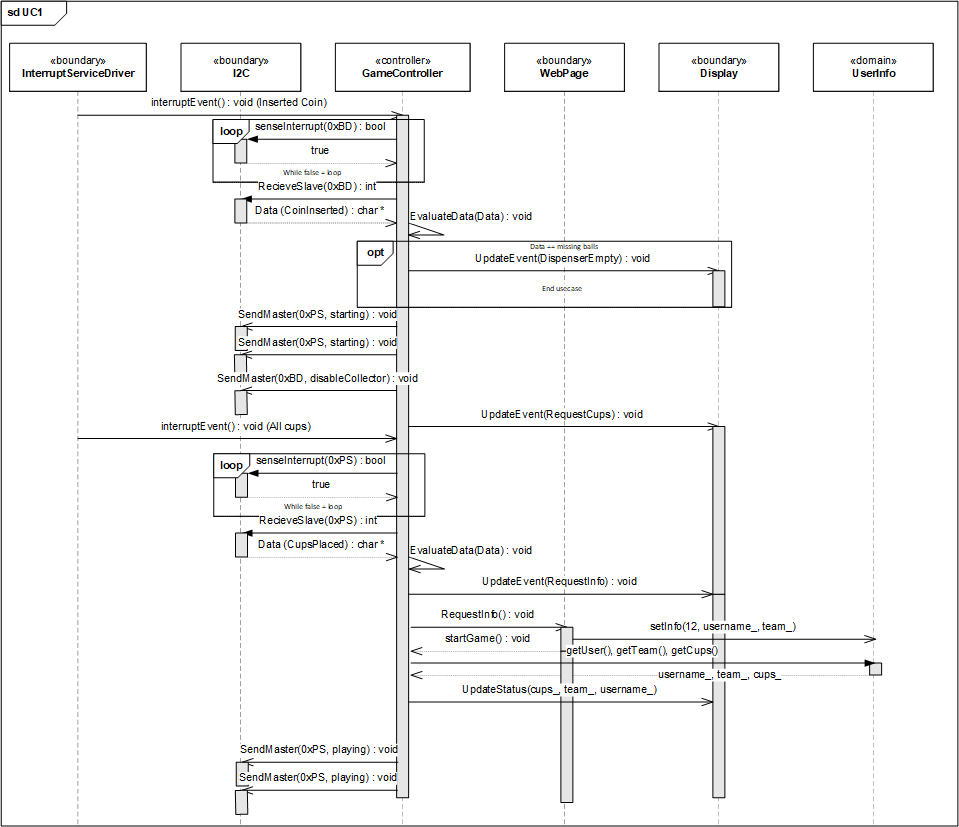
\includegraphics[width=\textwidth]{Arkitektur/Softwarearkitektur/Applikationsmodel/RPi/graphics_RPi/UC1_SD.png}
    \caption{Sekvensdiagram for UC1. Vær opmærksom på at mellemrummet mellem eksekverings specifikation 'boksen' indikerer en pause i processen; fx processeson 'sover', når der læses fra \textbf{BallDispenser} fx hvor der ventes information fra WebPage}
    \label{fig:UC1_SD_RPi_RAP}
\end{figure}
GameControllers tilstandsmaskine afspejler alle systemets tilstande. 
\begin{figure}[H]
    \centering
    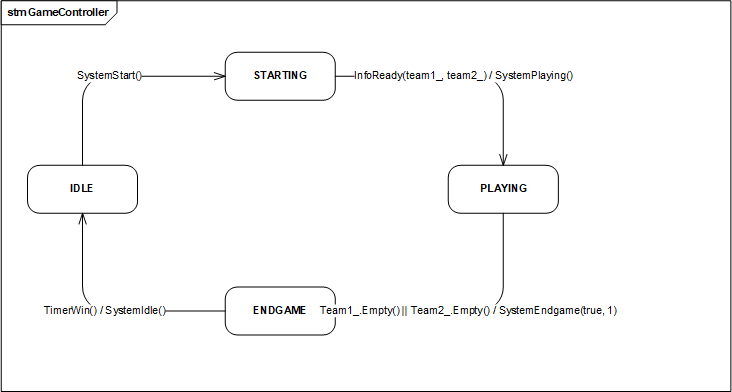
\includegraphics[width=\textwidth]{Rapport/Arkitektur/graphics/GAME_STATE.png}
    \caption{Tilstandsmaskine for GameController}
    \label{fig:STM_GAME}
\end{figure}
Read og write operationerne i userspace er tilknyttet en kernelspace driver. Device driveren er linket mellem det integrerede hardware i Rasberry Pi W Zero og userspace applikationen - driveren beskrives kort i det næste afsnit. 

\subsubsection{i2c\_interruptDriver}\label{sec:rap_i2c_intdriver}
I2c\_interruptDriver er den driver, som bruges på RPi'en. Den sørger for at sende beskeder og læse fra de forskellige PSoC's i systemet. På figur \ref{fig:driver_sekvensdiagram} ses sekvensdiagrammet for driveren. 
\begin{figure}[H]
    \centering
    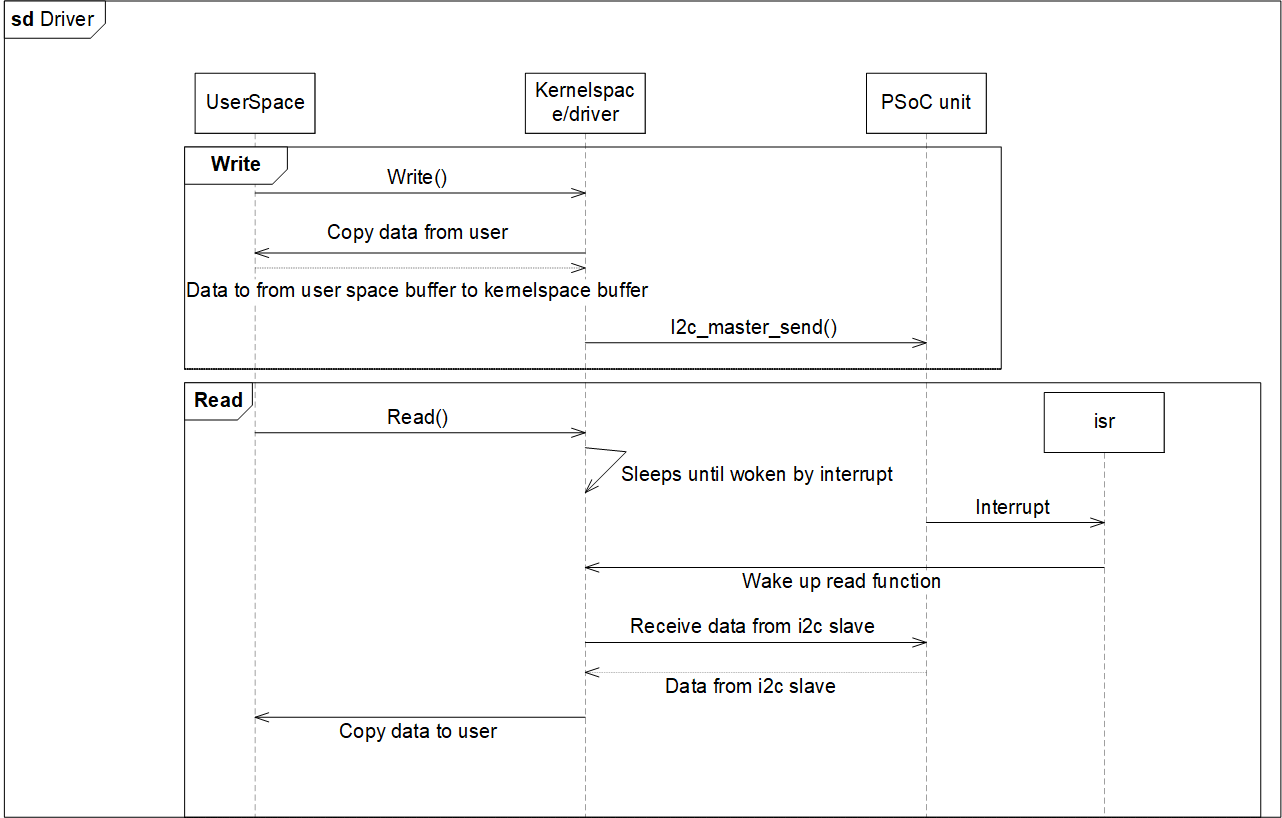
\includegraphics[width=\textwidth]{Rapport/Arkitektur/graphics/driver_sekvensdiagram.png}
    \caption{Her ses sekvensdiagram for driver, hvor samspillet mellem userspace, kernelspace og PSoC's(I2C slaver) vises.}
    \label{fig:driver_sekvensdiagram}
\end{figure}

\subsubsection{BallDispenserApp}
I dette avsnittet presenteres software arkitekturen for BallDispenser, for den fulle dokumentasonen refereres der til afsnittet \fullref{arch:sec:balldispenser_application_model} i dokumentet \textbf{Systemarkitektur}. Applikasjonen er skrevet i C for å kunne kjøres på en PSoC. Under vil klasse, sekvens og tilstands diagrammene til UC1 og UC4 bli presentert.\\\\


\textbf{Balldispenser - State machine}\\
\begin{figure}[H]
    \centering
    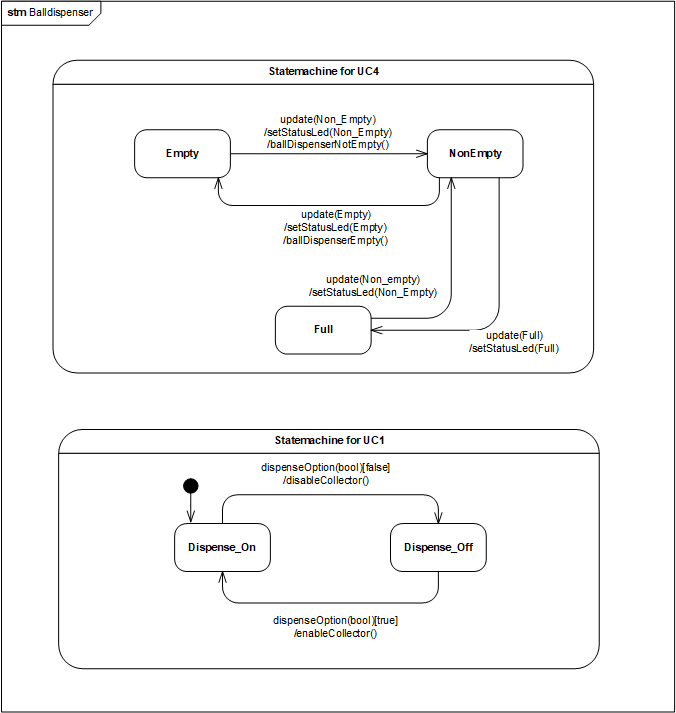
\includegraphics[width=\textwidth]{Arkitektur/Softwarearkitektur/Applikationsmodel/BallDispenser/graphicsBallDispenser/ApplikationsmodelBolddispenserstm.PNG}
    \caption{BallDispenser State machine}
    \label{fig:ball_dispenser_app_stm}
\end{figure}
Denne figuren viser stadiene for BallDispenser. Den består av to mindre state machines, en som styrer balldispenser og en som styrer CoinDispenser. CoinDispenser enable/disable styres av RPi via I2C. BallDispenser STMen styres av countBalls funksjonen. Dette dokumenteres grundigere i \textbf{Systemarkitektur} \fullref{arch:sec:BallDispSTM}.

\textbf{Sekvensdiagram for UC1}\\
\begin{figure}[H]
    \centering
    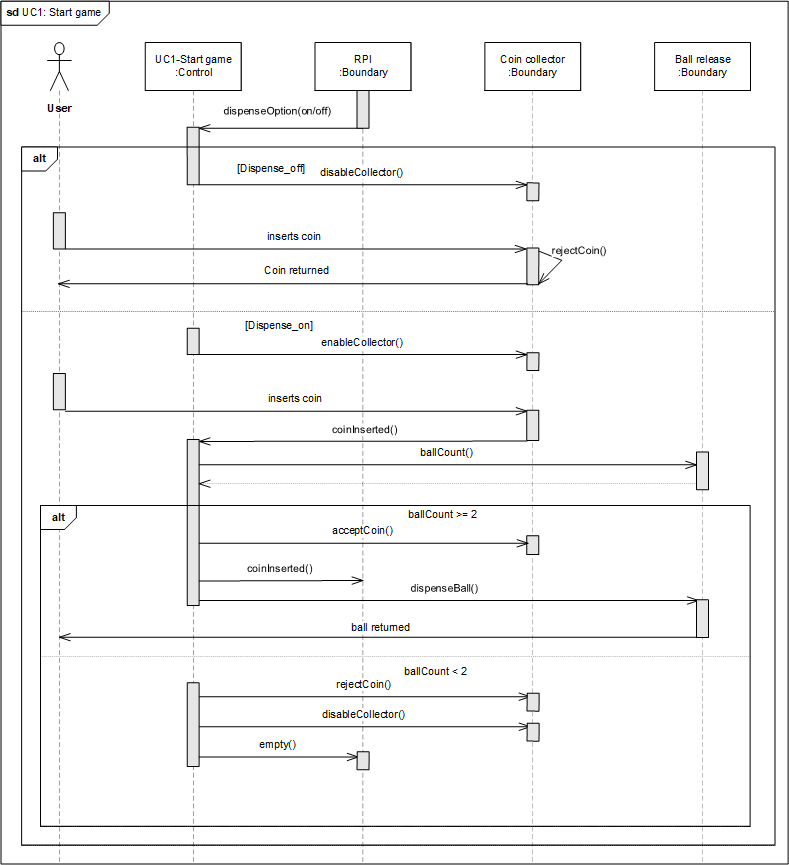
\includegraphics[width=\textwidth]{Arkitektur/Softwarearkitektur/Applikationsmodel/BallDispenser/graphicsBallDispenser/sdUC1.png}
    \caption{Sekvensdiagram for UC1 (Balldispenser)}
    \label{fig:BallDispScUC1}
\end{figure}

Ut fra sekvensdiagrammet (figur \ref{fig:BallDispScUC1}) kan det sees hvis en bruker innsetter en mynt i systemet mens det er i staten dispense\_off så kalder den rejectCoin() og fortsetter å vente. Mens hvis den er i dispense\_on skjekker den hvor mange baller som er igjen, hvis det det er nåkk akseperer den mynten, sender en beskjed til RPi og dispenserer baller. Hvis det ikke er nåkk avviser den mynten, disabler CoinCollector og sender beskjed til RPI.\\\\

\textbf{Sekvensdiagram for UC4}\\
\begin{figure}[H]
    \centering
    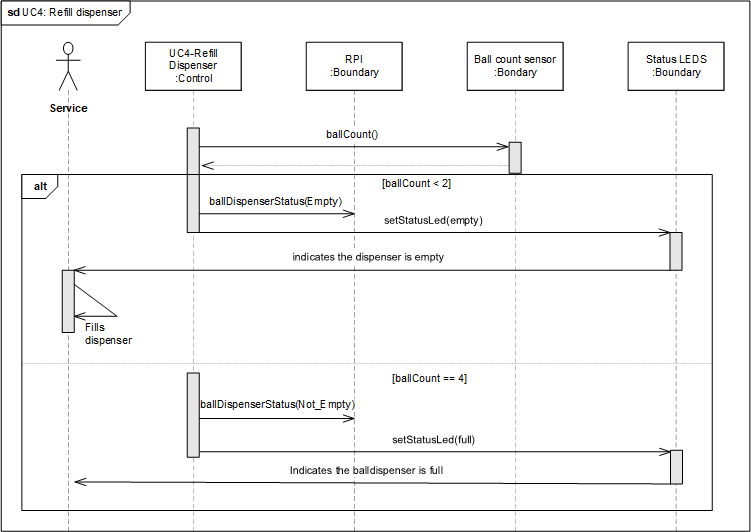
\includegraphics[width=\textwidth]{Arkitektur/Softwarearkitektur/Applikationsmodel/BallDispenser/graphicsBallDispenser/sdUC4.png}
    \caption{Sekvensdiagram for UC4 (Balldispenser)}
    \label{fig:BallDispScUC4}
\end{figure}

Ut fra sekvensdiagrammet (figur \ref{fig:BallDispScUC4}) kan det sees den starter med ballCount(), hvis den returnerer en verdi som er lavere enn 2 sender den beskjed til RPien om at den er tom og indiker det til service medarbedidern ved å endre på status LEDene. Etter dispenseren har blitt fylt kalles ballCount() igjen og LEDene endres slik de viser dispenseren er full.

\end{document}